\chapter[Hybrid Quantum-Classical Algorithms]{Hybrid Quantum-Classical\\Algorithms} \label{chap:hybrid-quantum-classical-algorithms}
At the end of the previous chapter, two important quantum algorithms were reviewed: the \gls{qft} and Grover's algorithm.
These quantum algorithms and the family of algorithms built on them require large-scale quantum computers with low error rates and high coherence.
The \gls{nisq} devices that are being built now and in the near future will not be able to run these algorithms.
To this end, \acrfullpl{hqca} that utilize both classical and quantum resources are being researched and developed.
This chapter will first introduce the basic concepts of \glspl{hqca} followed by a review of well-known and promising \glspl{hqca}.

\section{Basic Concepts}
\Acrlongpl{hqca} account for the limited number of qubits, limited connectivity of qubits, and limited coherence times of \gls{nisq} devices.
These algorithms often make use of the variational method which consists of preparing an initial trial state $\ket{\psi(\vec{\theta})}$ parameterized by real-valued parameters $\vec{\theta}$, and finding the parameters for which the expectation value of some observable is the lowest.
This family of \glspl{hqca} is sometimes also referred to as variational quantum algorithm, as it uses the variational method of quantum mechanics.

The general structure of a variational \gls{hqca} is shown in \Cref{fig:vqa-general-structure}.

\begin{figure}[ht]
    \centering
    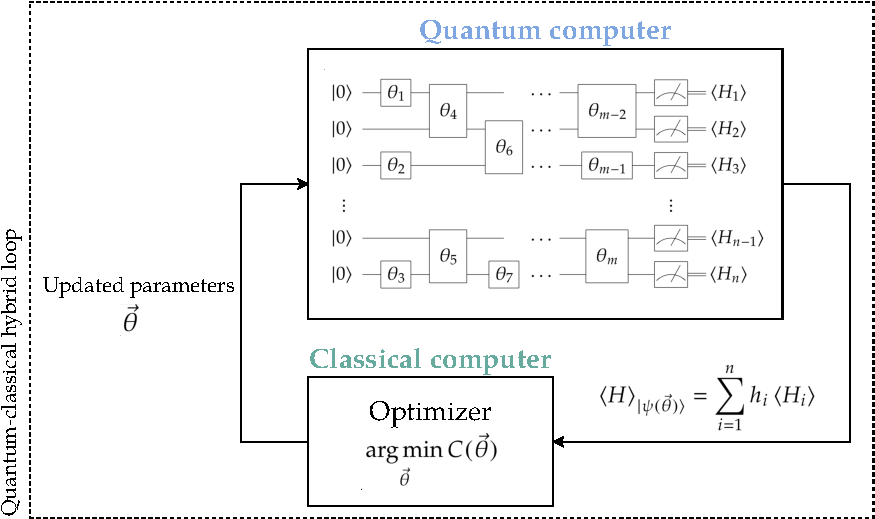
\includegraphics[width=1\linewidth]{figures/vqa-general-structure.pdf}
    \caption[The general structure of a variational quantum algorithm.]{The general structure of a variational quantum algorithm.}
    \label{fig:vqa-general-structure}
\end{figure}


\section{Variational Quantum Eigensolver}

\section{Quantum Approximate Optimization Algorithm}